\subsection{High-contrast imaging with the apodizing phase plate}
\label{ssec:algo_app_imaging}

LM-band imaging data taken with the apodizing phase plate undergo the
same basic reduction as standard imaging data. %\TODO{Does this include
 % background subtraction or is the background %subtracted during the
 % ADI processing?} if there is background remaining the ADI will take care of it.



\begin{enumerate}
\item Locate the positions of the PSFs with respect to each other
  (dither correction).
  This is primarily done through the \ac{WFS-FS} position information.
  The positions of the PSFs are also measured in the images themselves as a verification.
\item Center the leakage PSF in the frames.
\item Extract the coronagraphic PSFs and combine them into a single
  cube (see Fig.~\ref{fig:app_psf_combine}). This combined cube has an almost continuous 
  360\degr\ dark zone with a narrow brighter strip in between the original 180\degr\ dark zones, which is included in the static mask of step 6.
\item Median combine the cube to obtain the reference PSF image.
\item Subtract PSF image from all layers of the cube.
\item Derotate all layers to correct for field rotation, taking into
  account a static mask to reject noisy border regions of the dark
  zones.
\item Sum the layers to obtain final image.
  Intermediate data products are also provided.
\end{enumerate}

Additionally a reduction process where the two PSFs are handled separately also works. This will use the same approach however the mask will cover a larger angular extent.

\begin{figure}
  \centering
  \resizebox{0.8\textwidth}{!}{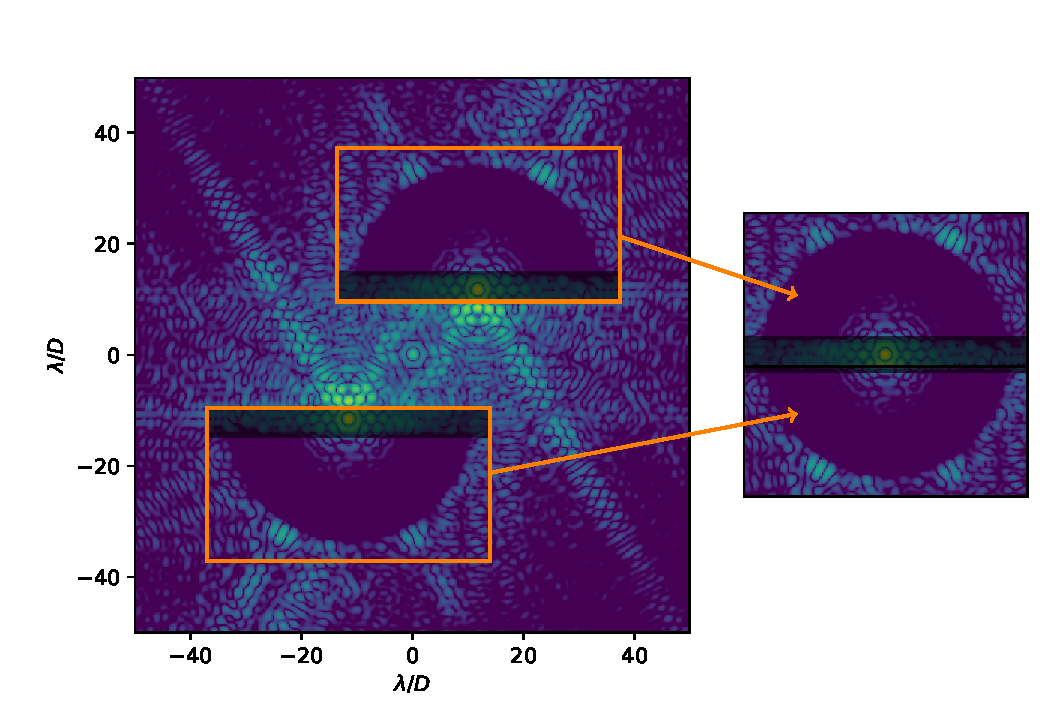
\includegraphics{APP_psf_combination}}
    \caption[Combination of the coronagraphic PSFs of APP observations into a single PSF]{%
        Combination of the coronagraphic PSFs of APP observations
        into a single PSF with nearly 360\degr\ dark zones. The bright
        horizontal stripes through the peak of the PSF will be masked for
        ADI post-processing.}
  \label{fig:app_psf_combine}
\end{figure}

%%% Local Variables:
%%% TeX-master: "METIS_DRLD"
%%% End:
